\chapter{The Internet Of Things}
\label{sec:IoT}
The Internet of Things (IoT) is a paradigm to which we put more and more attention in the scientific community.
It comes as a necessity, since new services must be provided to the new era of \textit{\textbf{"Smart Things"}}, which leverages existing infrastructure and communication technologies.
Such \textit{Smart} capabilities of future facilities will bring a radical change in human relationships with his everyday environment.
Moreover, most of the efforts to create this new services for people should focus in the seamless integration of new technologies, following the vision of ubiquitous computing proposed by Mark Weiser\cite{weiser1999ubiquitous}.
Yet humans will interact with this IoT infrastructure, their activity should be limited to the activation/deactivation of services, as well as a very small amount of configurations.
This systems are already present in everyday's life, such as sensor networks in smart cities, personal smartphones, RFID tags in most of retail stores, and so on.
However, this seamless integration still have several issues, from the development and deployment of services, to the usability.

\todo{develop more}

Some organizations, like the IEEE\footnote{IEEE, towards an IoT definition http://goo.gl/u4AjEd}, are proposing a complete definition to the IoT, but it is hard to have a common consensus.
However, for this thesis I will propose a definition from my experience and my own understanding, also based in those definitions.

\section{The IoT at a glance}
Nowadays, the current Internet, or the Internet of people, is driven by a set of technologies which were developed, extended and improved for the sake of human beings.
This \textit{\textbf{classical}} Internet technologies are those which are used, for instance, in computers, tablets, smart-phones, smart TVs and streaming boxes, just to name a few.
Users reach this Internet in form of web pages, audio and video streaming, mobile applications, and so on.
In the literature, these are called \textit{\textbf{web services}}, which are provided from other machines known as \textit{\textbf{web servers}}.
Web technologies are very well standardized, which allows a direct use of this information for any device implementing such standards.

On the other hand, systems that does not provide direct communication to the user, but on the contrary, communicate exclusively with other machines, should use different means to reach the Internet.
For this, a new infrastructure that provides connectivity to devices of this kind is necessary, and must leverage, as much as possible, existing frameworks to ease their integration and exploitation.
That's why the Internet of Things make use of different approaches, since the nature of their data and provided services differs significantly from classical web services.
The \textit{\textbf{web of things}}\cite{duquennoy2009webofthings} is the goal to achieve for this new infrastructure.

\section{Towards an infrastructure for IoT}
\label{sec:IoTInfra}
An IoT infrastructure can be defined as a set of interconnected objects that leverage one or more Internet protocols, in order to exchange information about the tasks for which they were programmed.

This infrastructure must be ready to support connectivity and interoperability for a huge number of devices of all nature, from a very small sensor to the cloud.
Furthermore, a compatibility with the current Internet basis should be developed, in order to take advantage of its robustness.

Existing deployments similar to the described above, such as smart cities, can serve as an example of the large scale this systems could reach.

\todo{start with the smart city example}


I highlight \textit{classical} because interoperability between objects is easier to achieve using the Internet infrastructure that already exists.
However, the objects participating into this new infrastructure could not be able  to run the existing Internet protocols implementations, since the available hardware resources can vary from an object to another.

The choice of the hardware is driven by the use we make of it, since the application could require an specific placement and connectivity.
The usage of this objects can be very varied, from common sensing/actuating tasks (temperature, humidity, air quality, HVAC, access control) to small algorithms that provide basic functionalities, such as thermostats, coffee machines, traffic monitors, and so on.
For instance, objects used for environmental sensing applications often need to be installed at a specific place\cite{younis2008placement}, which can be hard to reach. 
This forces to either reach the sensors with a specific cable, for both power and network connectivity, or use wireless communications.
On the other hand, for other devices like home appliances or smart meters, the placement is often already defined, and they can be easily connected to an existing network.

For the first kind of applications I mentioned above, wireless communications seem to be very convenient, while in the second example, a wired connection can already exist or could be easy to provide.
The communication method can determine the way we power the device, either using batteries or the electricity network.
Thus, two kind of objects with different hardware capabilities can be present in an IoT infrastructure, which we can separate into constrained and non-constrained.

Non-constrained devices\cite{RPi} are often able to run modern implementations of Internet protocols, since the hardware capabilities provided by objects powered by the electricity network are usually high.
Constrained devices\cite{iotlab-m3}, which are battery powered, does not provide enough computational resources to implement current Internet protocols \textit{as is}.
However, they provide more flexibility of installation, due to their physical size and cost.

\subsection{Very constrained resources: a scientific challenge}
The computational resources such as memory, can vary from a tens of bytes for low-cost microcontroller (MCU) based objects, to hundreds or thousands of mega bytes in both ROM and RAM for System on a Chip (SoC) based objects.

\begin{figure}[htb]
	\centering
	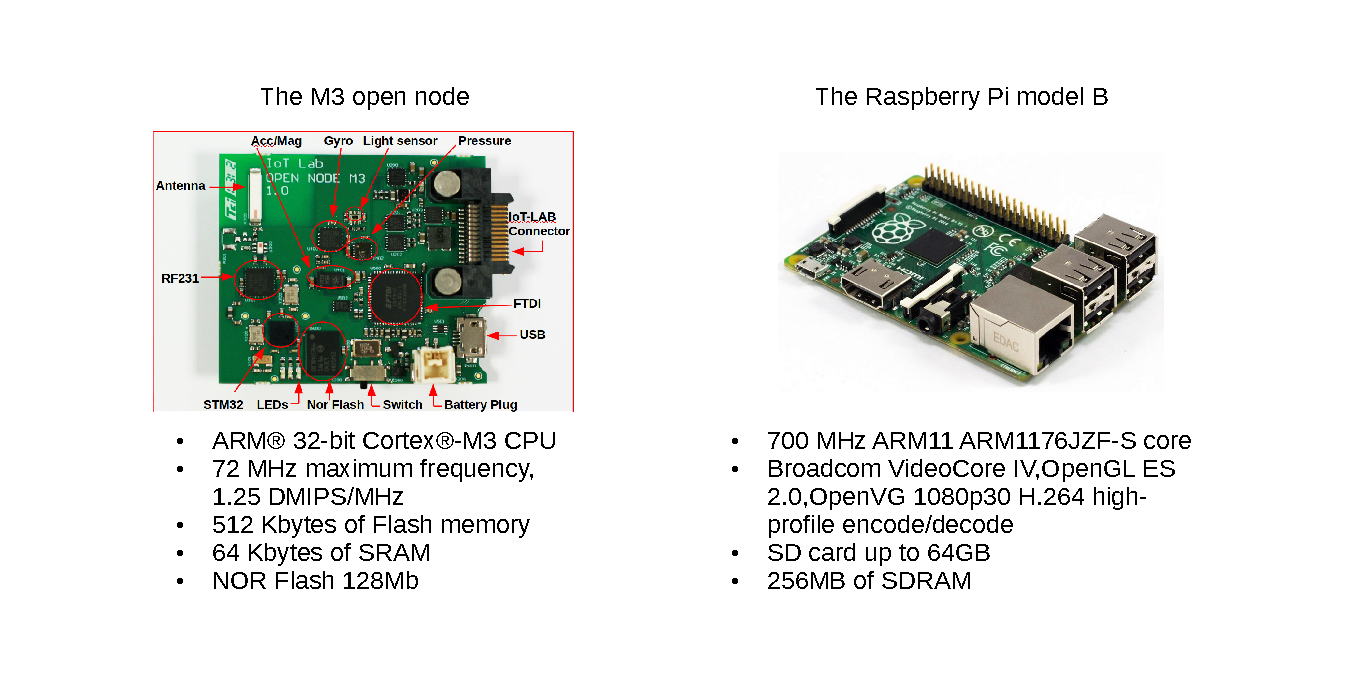
\includegraphics[width=1\columnwidth]{chapters/background.images/BoardsComparison.pdf}
	\caption{Constrained vs. non-constrained device}
	\label{fig:BoardsComparison}
\end{figure}

Figure \ref{fig:BoardsComparison} shows a resource comparison between this two kind of objects.
We can appreciate the big difference between them, as much in memory as in processing speed.
While the price and the resources of SoC systems is very attractive, power consumption still a main drawback.
Such kind of devices wouldn't last a day running in batteries, since the big amount of memory and the high speed processor are very power consuming.

The very low-cost of MCU based objects, coupled with their very low-power capabilities, make them very easy to produce and could be spread in most of physical environments, such as forests, streets, buildings and homes, since it is possible to make them run in batteries.
We can call this objects \textit{\textbf{smart objects}}.

In this thesis, I will put emphasis on MCU based smart objects, since most of the scientific challenges come with the constrained resources in memory and energy of such devices.

\subsection{Why smart objects are too resource constrained?}
This question arises when complex software developments are required to solve the "typical" problems already found in the classical Internet, that also exist in the IoT.
Web technologies are nowadays well investigated and offer many tools for fast development and maintenance, however, they rely in modern equipment: fast microprocessors with many cores, tens of gigabytes in RAM and several terabytes in hard disks.
While computers, mobile phones, and similar devices grow constantly in computing capacities, for microcontrollers the evolution is much less evident.
This avoids the use of most of already developed technologies, since the differences between this two kind of devices is enormous.
One of the main reasons for this, is the cost of MCUs.
In order to maintain a very low price for this devices, the size of them should be kept small.
Since SRAM (the volatile memory type used in MCUs) takes a lot of space in the chip, it is not possible to add more without increasing the cost of the chip, which is not wanted in a very competitive market as MCUs is.
In addition, the fabrication process of MCUs differs in many ways in comparison to SRAM construction.
Thus, for semiconductor foundries a complex device fabrication leads to an increased cost.
Finally, as we stated in section \ref{sec:IoTInfra}, in the IoT flexibility in the placement of IoT devices is a major concern.
SRAM being very energy consuming, it wouldn't be possible to power large SRAM devices using batteries.
Thus, to summarize, the construction of MCUs with huge quantities of memory is not economically viable, as well as the energy performance would be decreased.

\section{Communication between smart objects}
Several communication protocols are used in the classical Internet.
Most of them are based on Ethernet\cite{ieee802.3}, in which a standard cable is needed for each participant in the network.
A wireless Ethernet protocol was also standardized, as known as IEEE 802.11\cite{ieee802.11}, providing the same features without the need of cables.
Other ways to reach the current Internet also exists, such as optical fiber, satellite and different radio standards, just to name a few.

Since the IoT aims to be ubiquitous, communication using cables would complicate the physical installation of such objects.
The main advantage of MCU based objects is their very low power consumption.
Thus, a very low power communication interface would allow this objects to be powered using batteries.
Therefore, wireless communication protocols seem to be the best choice.
However, communication interfaces implementing standards i.e. IEEE 802.11, were not built having low power features in mind, making them too inefficient if batteries are used as power source.
Several wireless devices manufacturers and research institutes worked together to create new energy-aware protocols to provide wireless communication for smart objects.
One of the standards that came from these efforts was the IEEE 802.15.4\cite{ieee802.15.4}.
It was created specifically for low-power transceivers, allowing communication ranges near to 802.11, but offering a very low bandwidth.
This limitation avoid the exchange of large data packets, which also limits the protocols that can be managed by the interface, before having considerable fragmentation.

\begin{figure}[htb]
	\centering
	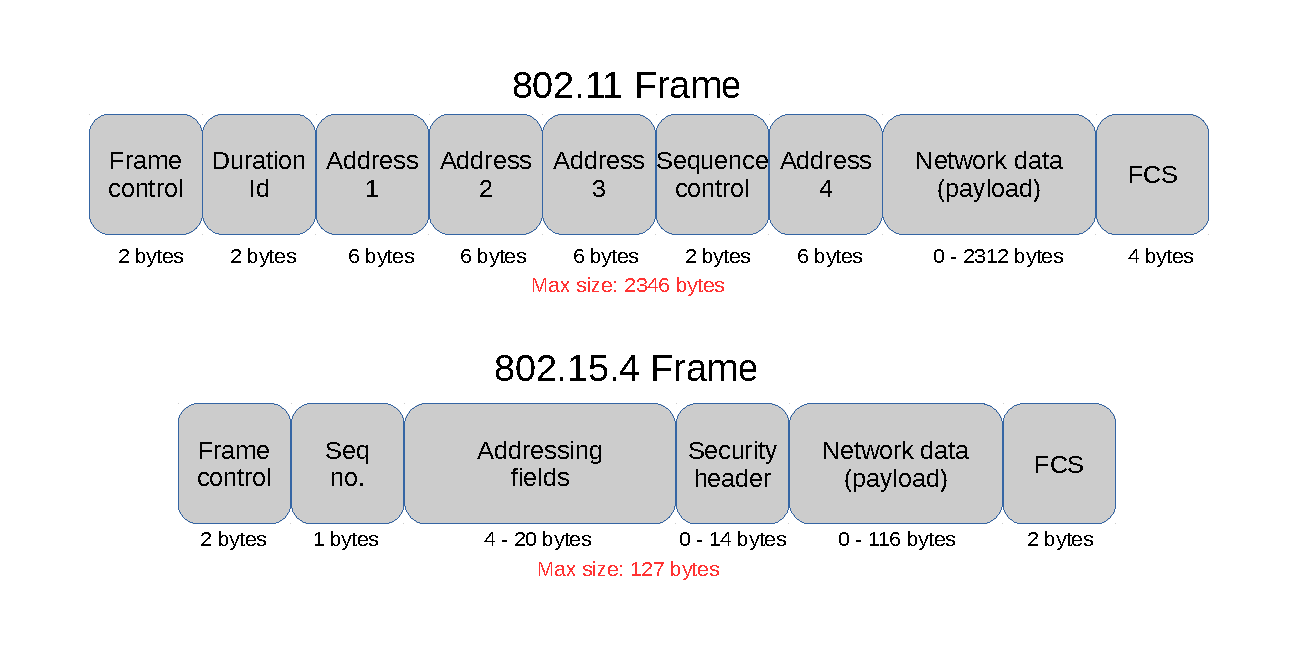
\includegraphics[width=1\columnwidth]{chapters/background.images/FramesComparison.pdf}
	\caption{Comparison in frame size between 802.11 and 802.15.4}
	\label{fig:FramesComparison}
\end{figure}

The memory constraints present in MCUs avoid the use of classical approaches to develop software for Internet based applications, often written in high level programming languages.
These approaches make use of common Internet protocol's implementations, which are not aware of this low resources.
Thus, a new way to provide Internet functionalities must be developed.

In 2003, Adam Dunkels developed a very lightweight TCP/IP protocol stack, uIP\cite{dunkels03full}, for 8-bit microcontrollers, enabling smart objects to communicate using a standard Internet protocol.
With this contribution, several services could be developed to create a first IoT infrastructure.
However, most of the services provided in classical Internet does not use a simple way to communicate, such as TCP/IP.
Therefore, a more complete framework for Internet services development should be created, to establish a more transparent and easy to use approach for resource constrained devices.

\subsection{6loWPAN, or how to give an IP address to any object}
With the arrival of the IPv6 standard\cite{rfc2460}, which enabled a wider range of IP addresses than the previous IPv4, the possibility to assign an address to each smart object became a reality.
This arise new challenges in the implementation for this new network protocol in smart objects, since the RFC2460 specification was intended for high resources machines.

Montenegro et al. proposed a new specification\cite{rfc4944} for constrained resources devices in order to communicate using IPv6 addresses.
This specification, called 6loWPAN (IPv6 for low-power Wireless Personal Area Networks) was successfully implemented\cite{durvy08making} and was able to provide interoperability with IPv6 ready devices, as it fulfilled all the requirements to have an IPv6 label\footnote{https://www.ipv6ready.org/}.
The main feature of the loWPAN adaptation layer is the compression of the IPv6 header, along with fragmentation and mesh addressing features.

\begin{figure}[htb]
	\centering
	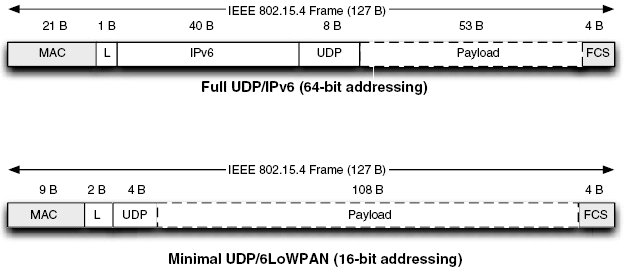
\includegraphics[width=1\columnwidth]{chapters/background.images/6lowpanvsipv6.jpg}
	\caption{IPv6 vs. 6loWPAN \cite{shelby2010embedded}}
	\label{fig:IPv6vs6loWPAN}
\end{figure}

A size comparison is done in figure \ref{fig:IPv6vs6loWPAN}.
We can appreciate that the header compression done by 6loWPAN reduces considerably its size, which is very important, given the size of IEEE 802.15.4 frames.

\begin{figure}[htb]
	\centering
	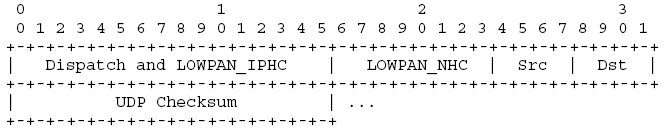
\includegraphics[width=1\columnwidth]{chapters/background.images/6lowpanDetails.jpg}
	\caption{6loWPAN header}
	\label{fig:6loWPANmin}
\end{figure}

In an ideal case, 6loWPAN headers can be as small as 6 bytes, shown in figure \ref{fig:6loWPANmin}.
This represents the "L" field in the frame.
\begin{figure}[htb]
	\centering
	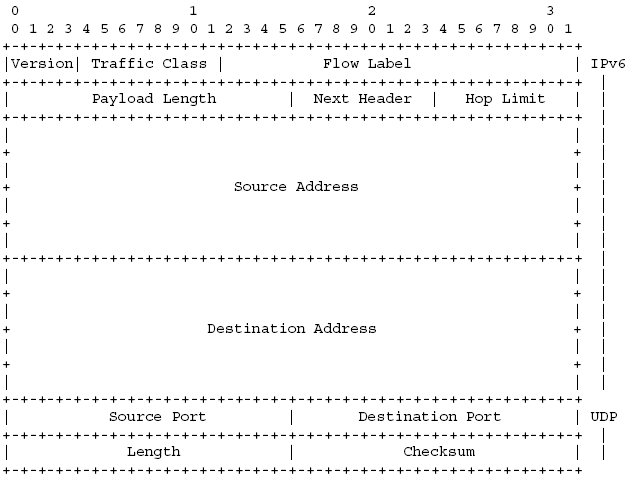
\includegraphics[width=1\columnwidth]{chapters/background.images/ipv6Details.jpg}
	\caption{IPv6 header}
	\label{fig:IPv6Header}
\end{figure}
As a comparison, the IPv6 header shown in figure \ref{fig:IPv6Header} would left only 72 bytes for payload, in the worse case.

Thanks to 6loWPAN compression, we have a first real \textit{"Internet of Things"} where every smart object can be reached from anywhere on Internet.
With this, we can think about web services, since the objects themselves can already be part of a network where they can offer their embedded services, hosted in their small amount of memory.
A new way to represent this services is then required, that could meet the current web services specifications and approaches.

\subsection{An application layer for smart objects}
In the classical Internet, web services are very often represented using the HTTP application protocol\cite{rfc2616}, in an architectural style called REST, defined by Fielding and Taylor\cite{Fielding02REST}.
REST services are very useful in the web, since they have a very easy way to operate using simple verbs: GET, POST, PUT, DELETE, just to name the common ones.
This representation could be also useful for smart objects, allowing the user, or other smart objects, to access its services in a standard way, providing interoperability with a good abstraction level.

While an implementation of HTTP is conceivable for smart objects, the huge amount of memory in both RAM and ROM turn it too heavy and inefficient to run on constrained, battery-powered devices\cite{Shelby10EWS}.
To solve this problem, Shelby et al. standardized the "HTTP for resource constrained devices"\cite{rfc7252}, called CoAP (Constrained Application Protocol).
This new application protocol is able to manage the methods described above, fulfilling the requirements for a RESTful API.
\begin{figure}[htb]
	\centering
	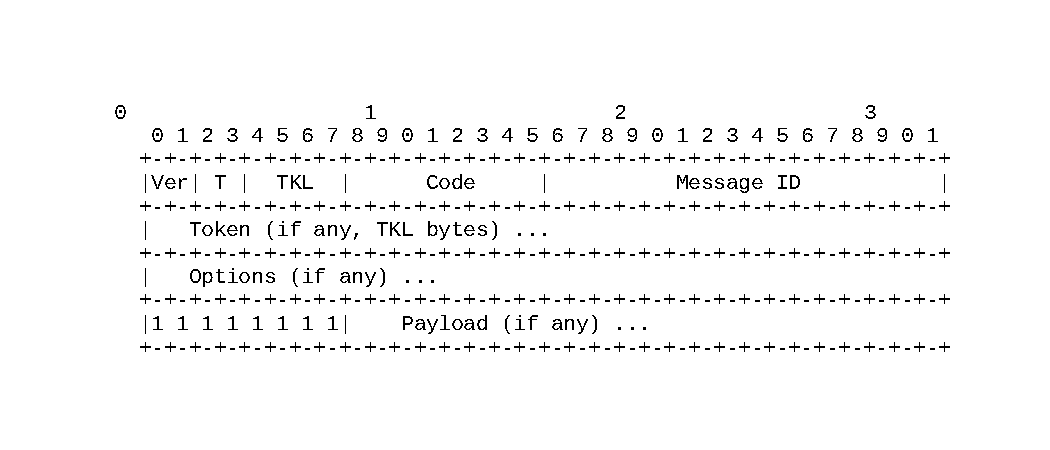
\includegraphics[width=1\columnwidth]{chapters/background.images/CoAPMessageFormat.pdf}
	\caption{CoAP Message format}
	\label{fig:CoAPMessageFormat}
\end{figure}
Figure \ref{fig:CoAPMessageFormat} shows a typical CoAP message, in which we can see that only 13 bytes are needed to format this message, allowing the rest of the frame for payload.

The services provided by the smart objects can be represented in a HTTP like form, i.e. \texttt{/sensors/temperature} for a temperature resource. If we use the CoAP command GET for this resource, we should have a response similar to "22.5", as an example of resource representation.
The PUT and POST commands are used to change the state of the actuators that can be present in a smart object.
For instance, if we want to change the state of a LED, we access the resource \texttt{/leds} with a query \texttt{?color=red} for a red LED, and a payload \texttt{mode=on} in order to turn it on.
This API facilitates the exchange of information between other smart objects, as known as "Machine to Machine (M2M)" communication.

CoAP was also developed having in mind the interoperability issue that comes when we need to communicate with other machines, which don't use CoAP as application protocol, providing an easy way to translate the messages to HTTP.

\section{Overview of the protocol stacks}
Having described a smart object capacities and capabilities, we can now make a layered comparison between the classical Internet and the IoT protocols stacks, built from the protocols already mentioned above.

\begin{figure}[htb]
	\centering
	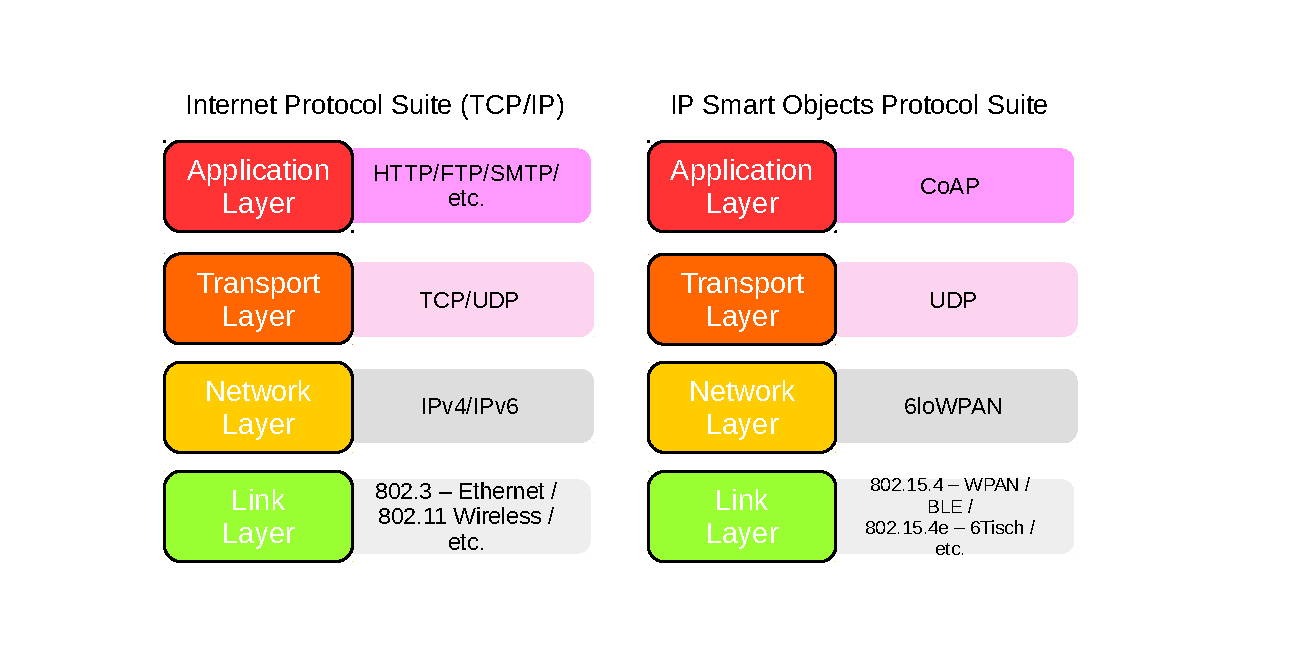
\includegraphics[width=1\columnwidth]{chapters/background.images/Layers.pdf}
	\caption{Comparison between Internet protocols stacks}
	\label{fig:IPLayers}
\end{figure}

In figure \ref{fig:IPLayers} we can appreciate a layered representation of both stacks, the classical Internet and the IoT.
This view allows a general understanding of some of the protocols that can enable an Internet of Things infrastructure.
Both stacks are able to communicate between them, allowing users and developers to mix different types of smart objects, as well as other types of devices that can participate in the same network, such as PC, servers and so on.

Nowadays, the establishment of so called \textit{"cloud services"}, forces to have standard communication protocols, since this services aim to be transparent to the users.
Thus, a standard network architecture is vital for the development, test, and continuous integration of web services.

\subsection{Other IP stacks for smart objects}
Other protocol stacks provide similar behavior than the mentioned above.
Several use privative protocols that limit the interoperability, which is very important when the connected smart objects to the IoT can reach several billions\footnote{http://www.cisco.com/web/solutions/trends/iot/portfolio.html}.
In the home and building automation domain, we can find for instance: BacNET/IP, KNX/IP, LonWorks/IP, and so on.
The wired communication bus used in these technologies, limits the possibility of spreading the objects in all environments, as described in section \ref{sec:IoTInfra}.
Although wireless specifications can exist for some of them\footnote{http://www.weinzierl.de/download/products/730/KNX\_over\_IP\_EN.pdf}, the IP connectivity is only achieved using specific routers that can encapsulate/de-capsulate the basic protocol for IP use.
Thus, there is no a transparent nor easy way to communicate with this objects.
This main drawback makes not viable the use of these protocols in an IoT infrastructure.

\section{IoT operating systems}
In the classical Internet several operating systems (OS) are used to take advantage of the services provided on the web.
An operating system provides all the necessary software to manipulate web content, based on user needs.
We can find, for instance, web browsers, mail clients, file managers, audio streamers, and so on, which use several Internet protocols already provided by the OS.

A similar need comes with the IoT.
However, web content in the IoT is not intended to be used directly by humans, but for other machines that gather such content and process it to offer new services.
Therefore, an operating system for the IoT should integrate all the necessary tools to provide a full communication stack, as well as a friendly environment to ease the development of applications.
In this section, some operating systems that provides such functionalities are described.

\subsection{Contiki}
Developed at the beginning for Wireless Sensor Networks (WSN) management, the Contiki OS\cite{dunkels2004contiki} provides a full network stack composed of several communication protocols, from the network to the application layers.
Built as a monolithic event-driven kernel, as well as modular, Contiki offers a standard way to develop applications, following a structured architecture of \textit{processes}.

Written in C, this OS and their applications can be compiled for several infrastructures, as Contiki provides enough abstractions to be platform independent.
The most common MCU architectures using this OS are msp430, AVR, ARM, among others.
The amount of memory needed in a 16-bit microprocessor (i.e. msp430) is about 2KB of RAM and 40KB of ROM.

\subsubsection{IoT protocol stack}
\begin{figure}[htb]
	\centering
	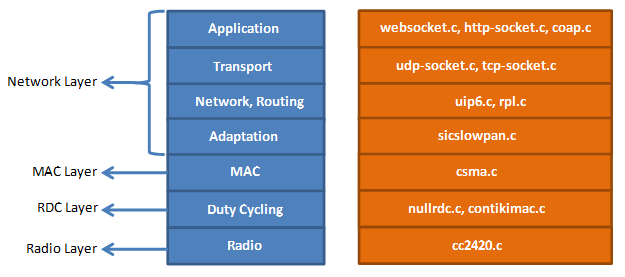
\includegraphics[width=1\columnwidth]{chapters/background.images/Contikinetstack.png}
	\caption{Contiki general network stack on the left (in blue) \& corresponding  netstack source codes on the right (in orange)}\footnote{Source files according to \url{https://github.com/contiki-os/contiki/tree/release-3-0}}
	\label{fig:ContikiNetStack}
\end{figure}
After several years of development, Contiki became an IoT OS by adding an IP Smart Object stack, which is described in figure \ref{fig:ContikiNetStack}.
Moreover, Contiki provides the following additional features:
\begin{itemize}
	\item Duty Cycling. ContikiMAC\cite{dunkels2011contikimac} is a radio duty cycling protocol that uses periodical wake-ups to listen for packet transmissions from neighbors.
	Since radio communication is the most energy consuming task, this feature reduces considerably the power consumption.
	\item MAC. An implementation of CSMA/CA that avoids collisions before sending a radio packet.
	\item Adaptation. SICSloWPAN is the Contiki implementation of the 6loWPAN RFC\cite{rfc4944}.
	\item Routing. ContikiRPL\cite{tsiftes2010contikirpl} implements the RPL\cite{rfc6550} protocol, which is an IPv6 Routing Protocol for Low-Power and Lossy Networks. RPL organizes a	topology as a Directed Acyclic Graph (DAG) that is partitioned into one or more Destination Oriented DAGs (DODAGs), one DODAG per sink.
\end{itemize}

\subsubsection{Mainly used features}
In addition to a very complete IP stack, Contiki integrates other useful features:

\begin{itemize}
	\item Multitasking kernel.
	\item Preemptive multi-threading.
	\item Proto-threads\cite{dunkels2006protothreads}.
	\item The RIME communication stack\cite{dunkels2007rime}.
	\item The Coffee file system\cite{tsiftes09enabling}.
	\item A dynamic loader of new modules\cite{dunkels06runtime}.
\end{itemize}

For this thesis, the Coffee file system and the dynamic loader were crucial for the experiments that validates this research work.

\subsubsection{The Coffee file system}
In a classical OS a file system is a mandatory feature.
Indeed, storing files and programs is one of the main functionalities that an OS can provide.
This is needed as much as for program execution, as for 


\subsection{RIOT}
RIOT is an IoT operating system\cite{baccelli2013riot}, with a microkernel architecture.
It supports a full IP stack for smart objects, offering interoperability with other OS like Contiki.
It's very low memory footprint make it idea for IoT, since it can be compiled for several architectures, from 8-bit to modern 32-bit microcontrollers.

google thread
manifeste usba

\section{Other embedded OS}
bla

\subsection{TinyOS}
bla
